
La carte du ciel suivante représente une portion de ciel visible pour un observateur se trouvant sur la Terre.

Le système de repérage s'appelle un \textit{repère équatorial}.

Les coordonnées se composent de l'ascension droite (en heure et minute) et de la déclinaison (en degré).

\begin{center}
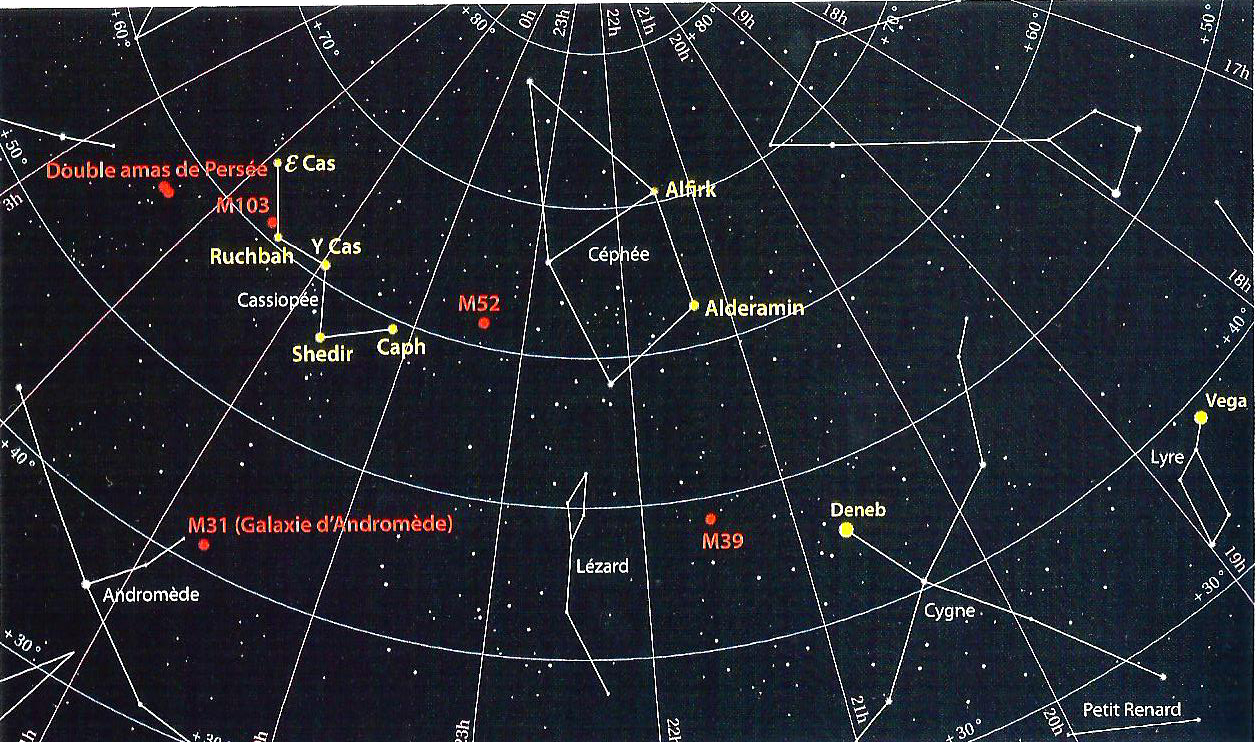
\includegraphics[scale=1]{ciel00.jpg} 
\end{center}


Déterminer de quelle partie du monde cette partie de ciel est visible.


\begin{minipage}{0.48\linewidth}

\subsection*{Dans la constellation de Cassiopée}

\begin{enumerate}
\item Quelle est la déclinaison de l'amas d'étoiles M103 ?
\item Quelle est la déclinaison de l'amas d'étoiles M52 ?
\item On a représenté ci dessous la constellation de Cassiopée, composée de 5 étoiles. La retrouver sur la carte et donner le nom de l'étoile qui possède la plus grande déclinaison.
\end{enumerate}
\end{minipage}
 \hfill
\begin{minipage}{0.48\linewidth}
\begin{center}
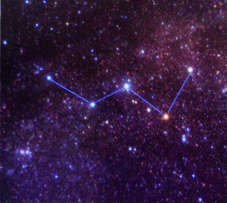
\includegraphics[scale=0.8]{ciel1.jpg} 
\end{center}
\end{minipage}



\subsection*{Dans la constellation de Céphée}

\begin{enumerate}
\item Quelle est l'ascension droite de l'étoile Alderamin ?
\item Quelle est l'ascension droite de l'étoile Alfirk ?
\end{enumerate}





\subsection*{Dans la constellation du Cygne}

Quelles sont les coordonnées de l'amas d'étoile M39 ?
\begin{center}
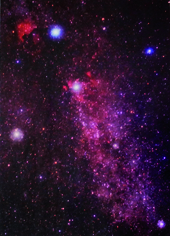
\includegraphics[scale=1]{ciel2.jpg} 
\end{center}

\subsection*{Avec des coordonnées}

Retrouver le nom des astres dont les coordonnées équatoriales sont :

\begin{enumerate}
\item (0 h 42 min ; 41$^o$) 
\item (20 h 41 min ; 45$^o$)
\item (2 h 20 min ; 57$^o$) ?
\end{enumerate}



